\documentclass{article}
\usepackage{tikz}
\usepackage{float}
\usepackage[paperheight=4.8in,paperwidth=7.3in,margin=-1in]{geometry}

\usetikzlibrary{fit,positioning,arrows.meta}
\begin{document}
\begin{figure}
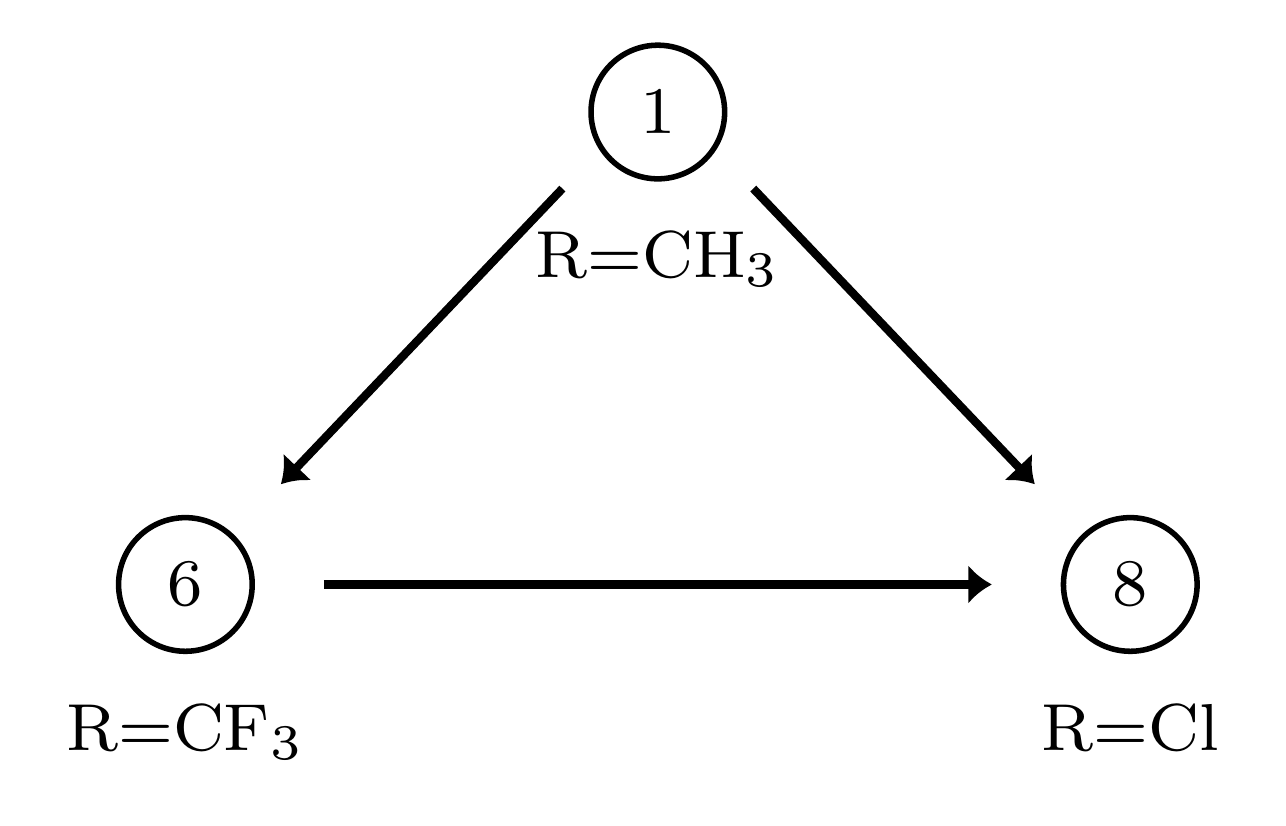
\begin{tikzpicture}[scale=3.0,transform shape,font=\footnotesize,node distance=2em]
  \node [circle,draw=black,line width=2pt] (l1_num) at (0,0) {1};
  \node [below=of l1_num.north] (l1_group) {R=CH$_3$};
  \node [fit={(l1_num) (l1_group)}] (l1) {};

  \node [circle,draw=black,line width=2pt] (l6_num) at (-2,-2) {6};
  \node [below=of l6_num.north] (l6_group) {R=CF$_3$};
  \node [fit={(l6_num) (l6_group)}] (l6) {};

  \node [circle,draw=black,line width=2pt] (l8_num) at (2,-2) {8};
  \node [below=of l8_num.north] (l8_group) {R=Cl};
  \node [fit={(l8_num) (l8_group)}] (l8) {};

  \draw [-{Latex[length=3mm,width=5mm]}, line width=3pt, shorten >= 5em, shorten <= 5em] (0,0.1) -- (-2,-2);
  \draw [-{Latex[length=3mm,width=5mm]}, line width=3pt, shorten >= 5em, shorten <= 5em] (0,0.1) -- (2,-2);
  \draw [-{Latex[length=3mm,width=5mm]}, line width=3pt, shorten >= 5em, shorten <= 5em] (-2,-2) -- (2,-2);
  % \draw [{Latex[length=3mm,width=5mm]}-, line width=3pt, shorten >= 5em, shorten <= 5em] (l1) -- (l6);
  % \draw [{Latex[length=3mm,width=5mm]}-, line width=3pt, shorten >= 5em, shorten <= 5em] (l1) -- (l8);
  % \draw [{Latex[length=3mm,width=5mm]}-, line width=3pt, shorten >= -12em, shorten <= -12em] (l6) -- (l8);
\end{tikzpicture}
\end{figure}
\end{document}


%%% Local Variables:
%%% mode: latex
%%% TeX-master: t
%%% End:
